\documentclass[11pt]{article}
\usepackage[utf8]{inputenc} % Para caracteres en espa�ol
\usepackage{amsmath,amsthm,amsfonts,amssymb,amscd}
\usepackage{multirow,booktabs}
\usepackage[table]{xcolor}
\usepackage{fullpage}
\usepackage{lastpage}
\usepackage{enumitem}
\usepackage{multicol}
\usepackage{fancyhdr}
\usepackage{mathrsfs}
\usepackage{wrapfig}
\usepackage[final]{pdfpages}
\usepackage{setspace}
\usepackage{esvect}
\usepackage{calc}
\usepackage{multicol}
\usepackage{cancel}
\usepackage{graphicx}
\graphicspath{ {pictures/} }
\usepackage[retainorgcmds]{IEEEtrantools}
\usepackage[margin=3cm]{geometry}
\usepackage{amsmath}
\newlength{\tabcont}
\setlength{\parindent}{0.0in}
\setlength{\parskip}{0.05in}
\usepackage{empheq}
\usepackage{framed}
%\usepackage{newtxmath}
\usepackage{euscript}
\DeclareMathAlphabet{\mathpzc}{T1}{pzc}{m}{it}
\usepackage[most]{tcolorbox}
\usepackage{xcolor}
\colorlet{shadecolor}{orange!15}
\parindent 0in
\parskip 12pt
\geometry{margin=1in, headsep=0.25in}
\theoremstyle{definition}
\newtheorem{defn}{Definition}
\newtheorem{reg}{Rule}
\newtheorem{exer}{Exercise}
\newtheorem{note}{Note}
\newcommand{\volume}{{\ooalign{\hfil$V$\hfil\cr\kern0.08em--\hfil\cr}}}
\newcommand{\parr}{\mathbin{\|}} % Parralel Symbol
\begin{document}
\setcounter{section}{0}
\setcounter{page}{1}
\setcounter{equation}{0}
\def\thepart{\arabic{part}}
\setcounter{part}{8}
\numberwithin{equation}{part}

 \pagestyle{fancy}
\fancyhf{}
\rhead{Section 8:  Electromagnetic Propulsion}
\rfoot{Page \thepage}
\thispagestyle{empty}

\begin{center}
{\LARGE \bf Section 8:  Electromagnetic Propulsion}\\
{\large AE435}\\
Spring 2018
\end{center}
%EM uses the lorentz force which makes them different from electrothermal thrusters.
EM thrusters create thrust by exploiting the Lorentz force:
 \begin{equation}
 \begin{aligned}
 \vv{F} = q \, (\vv{E} + \vv{v}\times \vv{B})
 \end{aligned}
 \end{equation}
 
In the simplest form can model this as two electrodes and a magnetic field:

\noindent\makebox[\textwidth]{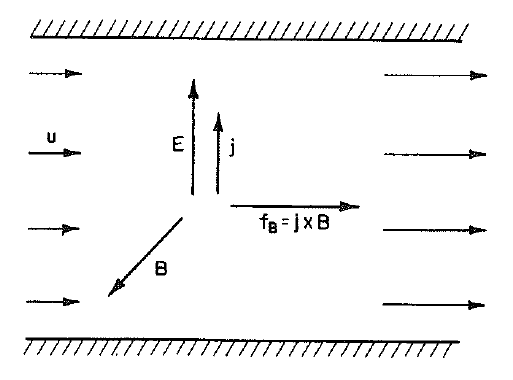
\includegraphics[scale=0.7]{1.png}}\\
You have an Efield created between anode and cathode. A Bfield out of the page which results in a ExB field. The current is going up the page and the ExB that pushes the plasma to the right. 

The physical mechanism from a particle point of view:

\noindent\makebox[\textwidth]{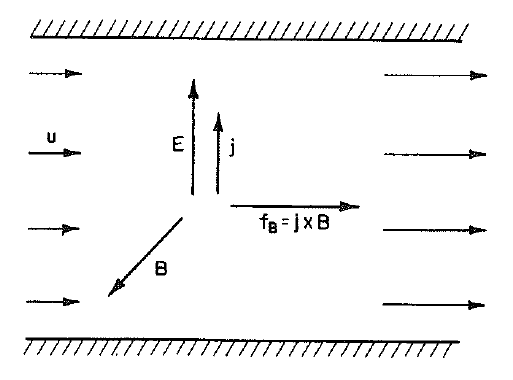
\includegraphics[scale=0.7]{1.png}}\\
Fluid stream, U, has electrons streaming from the cathode to the anode. Electrons streaming between the cathode and anode while picking up energy along the way. The ExB force causes them to gyrate. Collisions force everything out in the stream wise direction.
\begin{itemize}
\item Electrons steam from cathode to anode
\item Electrons pick up energy in Efield
\item Bfield sends electrons into gyration
\item Collisions result in preferential momentum transfer in streamwise direction
 \end{itemize}
\textbf{Types of accelerators:} \\
 \hspace{-10mm}\noindent\makebox[\textwidth]{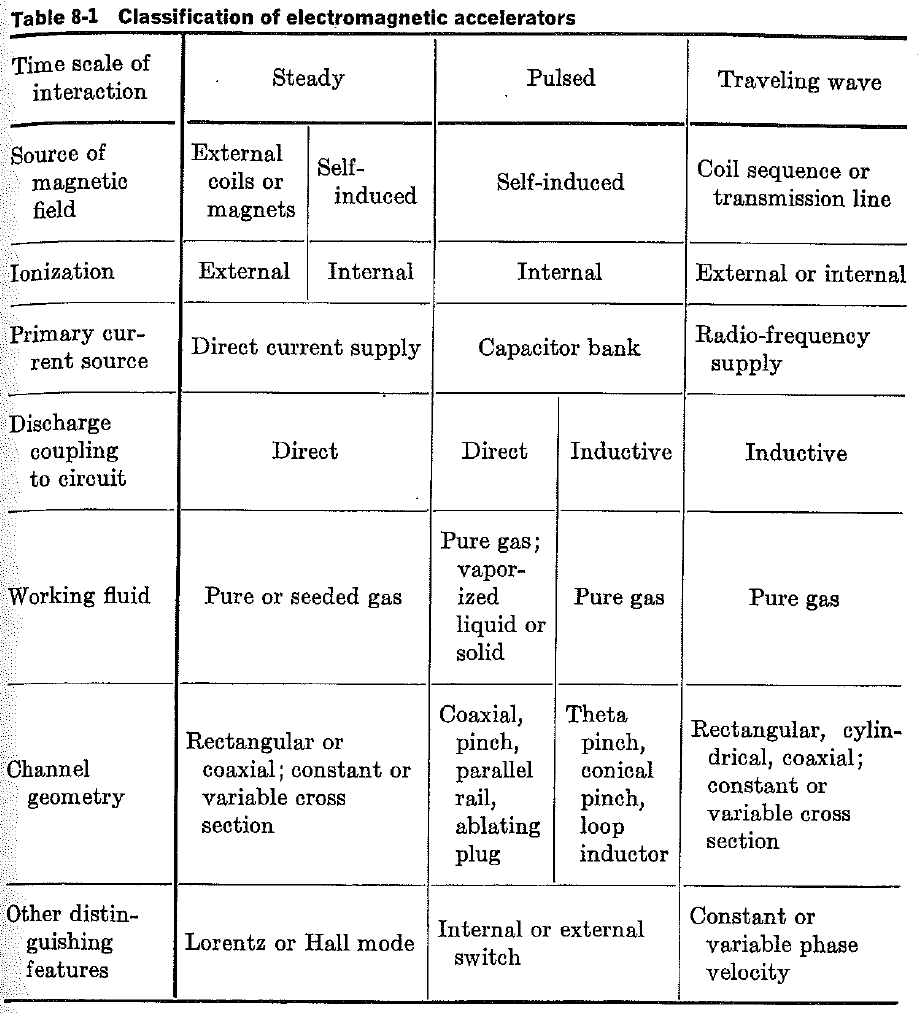
\includegraphics[scale=0.7]{3.png}}\\
 %From Jahn
 %Steady usual MPDT - often use a gas propellant. Work being done on a solid propellant
 %Pulsed usually PPT - often use teflon
 
Can be grouped by time scale of interaction:
\begin{itemize}
\item \textbf{Steady-state} - gasydnamics, electrodynamics, and thermal processes are all steady.
\item \textbf{Quasi-steady} - steady-state gasdynamics and electrodynamics, but not thermodynamics
\item \textbf{Pulsed} - transient discharges, accelerating slugs of gas
\item \textbf{Travelling-wave} - EM wave interacting with and accelerating plasma
 \end{itemize}
Since Bfield is strong enough to magnetize both electrons AND ions, the distinction between electrons and ions disappears from the equations.   We can use a \textbf{single-fluid} or \textbf{MHD (magnetohydrodynamic) model} to model this plasma: No distinction between ions and electrons. Simply jsut charged fluid.
 
\textbf{Continuity:}
 
  \begin{equation}
 \begin{aligned}
 \frac{\partial \rho}{\partial t} + \nabla \cdot (\, \rho \, \vv{u}) = 0
 \end{aligned}
 \end{equation}
 
\textbf{Equation of motion:}
 
  \begin{equation}
 \begin{aligned}
 \rho \, \bigg( \frac{\partial \vv{u}}{\partial t} + \vv{u} \cdot \nabla \vv{u} \bigg)= -\nabla p + \vv{j}\times \vv{B} + \vv{f}_v
 \end{aligned}
 \end{equation}
 JxB is the only thing that is different from what we seen previously since most fluid classes don't care about fluid effects.
 
\textbf{Energy balance}
 
  \begin{equation}
 \begin{aligned}
  \rho \, \bigg( \frac{\partial}{\partial t} + \vv{u} \cdot \nabla \bigg)\bigg(c_p \, T + \frac{u^2}{2}\bigg) =  \frac{\partial p}{\partial t} + \vv{j}\cdot \vv{E} + \phi_t + \phi_v - \phi_r
 \end{aligned}
 \end{equation}
Where

 \begin{equation*}
 \begin{aligned}
 c_p & = \text{Specific heat} \\ %Cp because open system we are interested in enthalpy witch accounts for both, the flow work  energy and internal energy. 
\phi_t & = \text{Net heat input by thermal conduction} \\
\phi_v & = \text{Net viscous dissipation} \\
\phi_r & = \text{Net power density for radiative losses"} \\
\vv{j}\cdot \vv{E} &\\
& \qquad  \text{Joule heating a dissipative (loss) term} \\
& \qquad  \text{Useful work caused by } \vv{F} \cdot \vv{v} \\
 \end{aligned}
 \end{equation*}
 
In Equation 8.4,  The left hand side represents time rate of change of energy inside the system. We are interested in internal energy and kinetic energy. The right hand side shows us what can cause this energy to change. Pressure, Work done by Efield, conduction, viscous dissipation, radiation emission from volume.
 
Also need equations of state for:
\begin{itemize}
\item Pressure, $P = P (\rho,T)$
\item Enthalpy, $h = h (\rho,T)$
\end{itemize}
As well as (tensor) transport coefficients for:
\begin{itemize}
\item Conductivity, $\sigma(\rho,T,E,B)$
\item Viscosity, $\eta(\rho,T,E,B)$
\item Thermal conductivity, $k$
\item Radiation
\end{itemize}
 
Only need 3 of Maxwell's equations since no qE term shows up in the equation of motion:
 %faradays law
 %maxwells law
 %___
   \begin{equation}
 \begin{aligned}
 \nabla \times \vv{E} &= -\frac{\partial \vv{B}}{\partial t} \\
 \nabla \times \vv{H} &= \vv{j} \\
 \nabla \cdot \vv{B} &= 0
 \end{aligned}
 \end{equation}
 
 
Can assume vacuum permittivity and vacuum permeability:
 
   \begin{equation}
 \begin{aligned}
 \vv{D} = \varepsilon_o \, \vv{E} \\ 
 \vv{B} = \mu_o \, \vv{H}
 \end{aligned}
 \end{equation}%Assume we have vacumm permitiviity and 
But Ohm's law has new terms:

   \begin{equation}
 \begin{aligned}
 \vv{j} = \sigma_o \, (\vv{E} + \vv{u} \times \vv{B}) + \vv{j}_H + \vv{j}_I
 \end{aligned}
 \end{equation}
Where

 \begin{equation*}
 \begin{aligned}
\vv{j}_H & = \text{Hall current (in jxB direction)} \\ 
& = \text{Has to deal with $E \times B$ drift, the importance is determined by the hall parameter.} \\ \\
\vv{j}_I & = \text{Ion slip (in (jxB)xB direction)} \\
& = \text{At low density and high B, ion-neutral collisions are rare so the ion velocity direction}\\
&\text{deviates or "slips" from neutral velocity direction. In most thrusters, the ion slip term is } \\
&\text{unimportant because we usually don't operate as low densities. }
 \end{aligned}
 \end{equation*}

%%These are the eqautions to model magentothruster

%We will now look at coaxial self field thrusters....

\end{document}